\chapter{Anhang}
\section{Loss-Function - Kreuzentropie}\label{anhang:kreuzentropie}
Diese Kreuzentropie lässt sich wie folgt beschreiben: \itenquote{Cross-entropy is a measure of the difference between two
probability distributions for a given random variable or set of events} \cite{machinelearningmastery:1:crossEntropy}.
Es ist also ein Mass, um die Differenz zwischen zwei Wahrscheinlichkeitsverteilungen einer Zufallsvariable oder einer
Menge von Ereignissen zu beschreiben. Um dies zu verstehen, wird zuerst die Entropie betrachtet. Diese beschreibt in der
Informatik die Anzahl Bits, welche benötigt werden, um ein zufällig gewähltes Element aus einer Wahrscheinlichkeitsverteilung
zu übertragen \cite{machinelearningmastery:1:crossEntropy}. Die Entropie kann weiterhin berechnet werden, wenn eine Menge
an Ereignissen $x$ in $X$ sowie deren Wahrscheinlichkeit $P(x)$ bekannt sind. Dies ist aus der Gleichung \ref{eq:ap:2} zu entnehmen.
\begin{align}
    H(P) = - \sum_{x \in X} P(x) \cdot log(P(x)) \label{eq:ap:2}
\end{align}
Die Kreuzentropie baut nun auf dieser Definition auf. Sie beschreibt die Anzahl Bits, welche benötigt werden, um ein
durchschnittliches Ereignis einer Wahrscheinlichkeitsverteilung im Vergleich zu einer anderen darzustellen \cite{machinelearningmastery:1:crossEntropy}.
Nun kann ein Ereignis $x$ in zwei Wahrscheinlichkeitsräumen vorkommen. Einerseits in $P$, andererseits in $Q$. Weiterhin
müssen die Wahrscheinlichkeiten der Ereignisse $P(x)$ und $Q(x)$ innerhalb dieser Verteilungen bekannt sein. Dadurch ergibt
sich die Gleichung \ref{eq:ap:3}.
\begin{align}
    H(P,Q) = - \sum_{x \in X} P(x) \cdot log(Q(x)) \label{eq:ap:3}
\end{align}
Wie genau ist dies nun im Kontext von Machine Learning zu verstehen? Grundsätzlich geht es darum eine Klassifikation vorzunehmen.
Dabei kennt man für ein Sample die Wahrheit. Diese Wahrheit zeigt sich in der Form der Wahrscheinlichkeitsangabe für eine Klasse.
Wenn es sich also z.B. um ein KNN handelt und dieses trainiert wird, um drei Klassen (Apfel, Birne, Zitrone) zu unterscheiden und
ein Sample \glqq Birne\grqq{} propagiert wird, dann ist die korrekte Wahrscheinlichkeitsverteilung $P$ (0, 1, 0), wohingegen
das KNN für dieses Sample ein anderes Resultat liefert, nämlich $Q$ (0.2, 0.7, 0.1). Nun kann für das Ereignis \glqq Birne\grqq{} die
Kreuzentropie über beide Wahrscheinlichkeitsverteilungen berechnet werden, um den Unterschied derer zu bestimmen.
Konkret bedeutet das für das aktuelle Beispiel:
\begin{align}
    H(P,Q) = - (P(Apfel) \cdot log(Q(Apfel)) + P(Birne) \cdot log(Q(Birne)) + P(Zitrone) \cdot log(Q(Zitrone)))\\
    H(P,Q) = - (0 \cdot log(0.2) + 1 \cdot log(0.7) + 0 \cdot log(0.1))\\
    H(P,Q) = - (1 \cdot log(0.7))\\
    H(P,Q) = - (-0.514573)\\
    H(P,Q) = 0.514573
\end{align}
Die Frage stellt sich nun, wieso diese Kreuzentropie sich so gut als Loss-Funktion eignet. Dazu muss bedacht werden, dass die
Entropie für eine Wahrscheinlichkeitsverteilung wie im Falle von $P$ des vorherigen Beispiels immer $0$ beträgt. Dies kann
sehr einfach anhand der Entropie gezeigt werden. Man nehme für die Wahrscheinlichkeitsverteilung $P$ für die Ereignisse $x_1 \cdots x_n$ die
folgenden Wahrscheinlichkeiten an: $(p_1, \cdots, p_k, \cdots, p_n)$ wobei $p_k = 1$ und $p_{i \neq k} = 0$ gilt.
Dadurch ergibt sich für die Entropie folgenden Formel:
\begin{align}
    H(P) = - (\sum_{i = 0}^{k - 1}(P(x_i) \cdot log(P(x_i))) + P(x_k) \cdot log(P(x_k)) + \sum_{i = k+1}^{n}(P(x_i) \cdot log(P(x_i)))) \label{eq:ap:4}
\end{align}
Aus der Formel \ref{eq:ap:4} ist ersichtlich, dass die erste wie auch die letzte Summe auf $0$ evaluieren, da die Wahrscheinlichkeit des Ereignisses $x_i$
jeweils $0$ ist. Einzig das Ereignis $x_k$ ist $1$, daher kann die Formel wie in \ref{eq:ap:5} gekürzt werden.
\begin{align}
    H(P) = - (P(x_k) \cdot log(P(x_k))) \label{eq:ap:5}\\
    H(P) = - (1 \cdot log(1))\\
    H(P) = - (1 \cdot 0)\\
    H(P) = 0
\end{align}
Nun gilt es noch zu beachten, dass die Kreuzentropie der Entropie entspricht, wenn es sich um dieselbe
Wahrscheinlichkeitsverteilung handelt. Dadurch wird klar, dass wenn ein Machine-Learning Algorithmus
ein Resultat einer Klassifikation berechnet, welches exakt mit der Wahrheit übereinstimmt, dies $0$ ergibt.
Das Sample wurde korrekt klassifiziert.\cite{machinelearningmastery:1:crossEntropy}.

\subsection{Binäre Kreuzentropie}\label{anhang:binary:kreuzentropie}
Besteht die Grundwahrscheinlichkeit $P(x)$ nur aus zwei möglichen Zuständen ($0$ oder $1$), dann kann die Formel der Kreuzentropie
vereinfacht werden. Zu Beginn sei angemerkt, dass zwei Wahrscheinlichkeiten angenommen werden können, welche zusammen
$1$ ergeben. In dem Fall $1 = P_1(x) + P_2(x)$. Da $P(x)$ binär ist, muss entweder $P_1(x)$ oder $P_2(x)$ $0$ sein.
Nun lässt sich $P_2(x)$ über die Gegenwahrscheinlichkeit von $P_1(x)$ ausdrücken. Siehe dazu die Formel \ref{eq:ap:6}
\begin{align}
    P_2(x) = 1 - P_1(x)\label{eq:ap:6}
\end{align}
Über die binäre Eigenschaft von $P(x)$ lässt sich die Kreuzentropie in dem Fall wie in Formel \ref{eq:ap:7} formulieren.
Anzumerken sei hier, dass wenn $P_1(x) = 1$ gilt, nur der Logarithmus des Wahrscheinlichkeitswerts $Q_1(x)$ von Bedeutung ist.
Wenn $P_2(x) = 1$ gilt, dann gilt automatisch $P_1(x) = 0$ und es ist nur noch der Logarithmus des Wahrscheinlichkeitswerts von
$Q_2(x)$ relevant. Es wird also jeweils die Abweichung der Wahrscheinlichkeiten $P_1(x)$ zu $Q_1(x)$ oder der Wahrscheinlichkeiten
$P_2(x)$ zu $Q_2(x)$ betrachtet.
\begin{align}
    H(P,Q) = - \sum_{x \in X} (P_1(x) \cdot log(Q_1(x)) + P_2(x) \cdot log(Q_2(x)))\label{eq:ap:7}
\end{align}
$P_1(x)$ sowie $Q_1(x)$ sind sehr natürlich, denn es ist klar, dass ein Sample $x$ eine Wahrscheinlichkeit
in beiden Wahrscheinlichkeitsverteilungen hat. Es irritiert aber, dass dort anscheinend zwei Wahrscheinlichkeiten für ein und
dasselbe Ereignis/Sample existieren sollen, also $P_2(x)$ und $Q_2(x)$. Diese Information wird nun tatsächlich nicht direkt in den
Wahrscheinlichkeitsverteilungen $P(x)$ und $Q(x)$ abgelegt, durch die Binarität von $P(x)$ sind sie jedoch durch die Formel
\ref{eq:ap:6} indirekt über die Gegenwahrscheinlichkeit gegeben. Siehe dazu Formel \ref{eq:ap:8}.
\begin{align}
    H(P,Q) = - \sum_{x \in X} (P_1(x) \cdot log(Q_1(x)) + (1 - P_1(x)) \cdot log(1 - Q_1(x)))\label{eq:ap:8}
\end{align}
Nun können in der Formel \ref{eq:ap:8} noch die Indizes der Wahrscheinlichkeitsverteilungen weggelassen werden, womit
die Endgültige Formel in \ref{eq:ap:9} entsteht.
\begin{align}
    H(P,Q) = - \sum_{x \in X} (P(x) \cdot log(Q(x)) + (1 - P(x)) \cdot log(1 - Q(x)))\label{eq:ap:9}
\end{align}
Dies kann nun folgendermassen interpretiert werden:
\begin{description}
    \item[$P(x) = 1$] In dem Fall wird die Abweichung zum Wert $1$ betrachtet. Daher wird der Wert aus $Q(x)$ übernommen.
    Das Resultat muss $0$ lauten, wenn $Q(x)$ ebenfalls $1$ ist.
    \item[$P(x) = 0$] Es wird die Abweichung zum Wert $0$ gemessen, was bedeutet, dass $1 - P(x)$ auf $1$ evaluiert und
    $\log(1 - Q(x))$ demnach $0$ ergeben sollte, wenn $Q(x)$ ebenfalls $0$ ist.
\end{description}

\section{Erwartungswert - arithmetisches Mittel}\label{anhang:erwartungswert}
Der Erwartungswert gibt den Durchschnitt der Ergebnisse einer Zufallsvariablen an.\cite{wiki:erwartungswert}
\begin{align}
    X = \{x_1, \ldots, x_n\}\\
    E(X) = \sum_{i = 1}^{n} (p_i \cdot X_i)
\end{align}
Wenn die Wahrscheinlichkeitsverteilung gleichverteilt ist, dann entspricht jede
Wahrscheinlichkeit $p_i$ derselben Wahrscheinlichkeit $\frac{1}{n}$.
Durch Ausklammern ergibt sich das arithmetische Mittel.
\begin{align}
    E(X) = \frac{1}{n} \cdot \sum_{i = 1}^{n} (X_i)
\end{align}

\section{Minimax}\label{anhang:minimax}
Um zu verstehen, wieso es sich hierbei um einen solchen Minimax-Algorithmus handelt, wird in diesem Abschnitt ebendieser mit
Verweis auf die Gleichung \ref{eq:1} eingeführt. Der Algorithmus geht auf den Versuch zurück, für ein Zwei-Spieler-Spiel eine
schlaue KI zu erschaffen, die möglichst weit in die Zukunft sehen und abschätzen kann, was der Gegener tun wird.
Dabei geht man davon aus, dass der Gegner immer so agiert, damit er seine Gewinnwahrscheinlichkeit maximiert und die
der KI minimiert.\cite{towardsdatascience:minimax} Die Züge, welche gemacht werden können, werden über einen sogenannten
Game-Tree dargestellt. Dieser ist in Abbildung \ref{fig:Berechneter GAN-Game-Tree} ersichtlich,
es ist der Game-Tree für ein \Gls{GAN} gegeben. Jeder Layer stellt einen Zug in diesem Spiel dar.
Innerhalb eines Zuges gibt es viele Möglichkeiten. Jede dieser Möglichkeiten wird über einen Node repräsentiert.
In der Gleichung \ref{eq:1} geht es um die Maximierung für $D$, weswegen die grünen Layer zu $D$ gehören. In diesen Zügen
soll der Algorithmus die Value-Funktion $V(G,D)$ für einen Node aus seinen Nachfolgern maximal wählen. Hingegen soll $G$ minimiert werden, weswegen
die roten Layer zu $G$ gehören. Innerhalb dieser Layer wird der minimale Wert der nachfolge States bevorzugt. Ist eine gewisse
Tiefe erreicht worden, oder es gibt keine Nachfolge-States mehr, dann wird die Value-Funktion $V(G,D)$ für diese States aufgerufen und für den
jeweiligen Status der Wert berechnet. Abbildung \ref{fig:Berechneter GAN-Game-Tree} zeigt einen möglichen ausgefüllten Game-Tree über drei Stufen hinweg.
\begin{figure}[h!]
    \begin{center}
        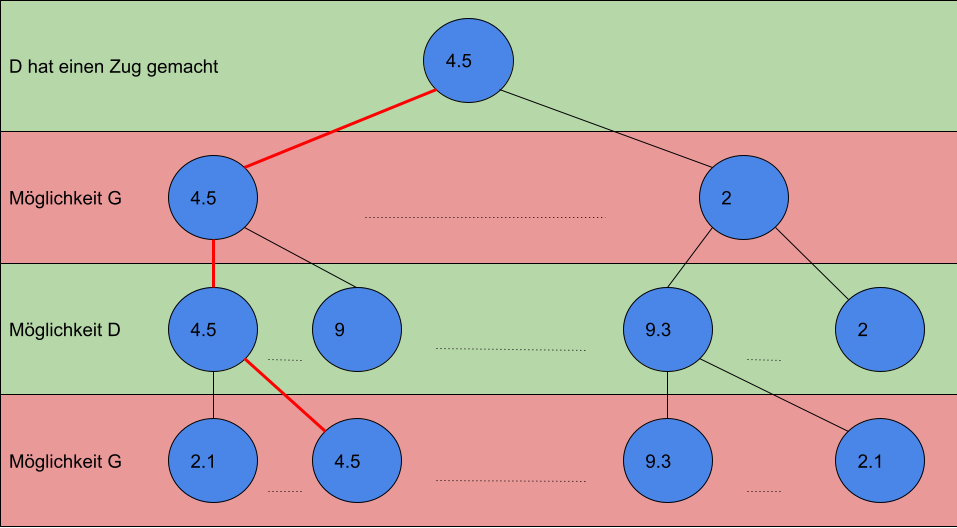
\includegraphics[width=0.5\textwidth]{../common/04_appendix/resources/00_gan_game_tree_filled.png}
    \end{center}
    \caption{Berechneter GAN-Game-Tree}
    \label{fig:Berechneter GAN-Game-Tree}
\end{figure}
Der rote Pfad bildet nach aktuellem Kentnisstand der beste Weg für $D$, und wird diesen wählen unter der Annahme,
dass $G$ wiederum den Weg wählen wird, welcher für $G$ am besten ist.

\section{Neuronale Netze - Multilayer Perceptron}\label{anhang:neuronale_netze}
Da die Architektur des \Gls{GAN} auf zwei neuronalen Netzen beruht, wird in diesem Kapitel kurz darauf eingegangen, wobei
nicht die Absicht besteht, ein vertieftes Wissen zu vermitteln.
\para
Die neuronalen Netze sind, wie so manches, über die Zeit herangereift. Die Intention besteht nicht darin, das menschliche Gehirn
nachzubauen, sondern eher eine Art Modell für die Informationsverarbeitung zu beschreiben \cite{wiki:knn}. Wie in der Biologie versucht man dies
in diesen Netzen über Neuronen, wo auch der Name herrührt. Ein solches
Neuron bekommt als Eingabe eine Summe von gewichteten Werten, welche es durch eine sogenannte \glqq Aktivierungsfunktion\grqq{} in
einen Ausgabewert umwandelt.
\para
Am Anfang dieser Netzwerke stand das Perzeptron, welches nur ein
einziges künstliches Neuron beinhaltet und von Frank Rosenblatt beschrieben wurde.\cite{wiki:perzeptron} Danach hat man damit
begonnen, diese Neuronen über Layer miteinander zu verbinden, wobei man den ersten Layer als Input-Layer, die Layer dazwischen
als Hidden-Layer und den letzten Layer aus Output-Layer kennt. Der Output-Layer beinhaltet in einem einfachen \Gls{KNN} so viele
Neuronen, wie es Klassen gibt. Jedes dieser Output-Neuronen gibt die Wahrscheinlichkeit an, ob eine Eingabe zu der jeweiligen
Klasse gehört \cite{wiki:knn}.
\para
Ein solches neuronales Netz ist eigentlich eine Optimierungsaufgabe. In dem Fall geht es darum, am Ende eine Fehlerfunktion, welche
den Abstand des Ist- und Sollzustands beschreibt, zu minimieren. Je geringer der Fehler, desto besser klassifiziert das Netz. Die
Variablen, welche dabei angepasst werden können, sind die Gewichte, welche jeweils auf einer Verbindung zwischen zwei Neuronen liegen.
Wie wahrscheinlich jeder aufmerksame Leser erkennt, werden dies sehr schnell sehr viele Variablen, weswegen normale Verfahren wie
z.B. der Gradientenabstieg zwar eingesetzt werden können, aber sehr ineffizient sind.
Der Durchbruch dieser Netzwerke wurde daher erst mit der Beschreibung des \Gls{Backpropagation}-Algorithmus erzielt, welcher ein Spezialfall
des Gradientenabstiegverfahrens darstellt und die Gewichte aufgrund ihres Anteils am Fehler anpasst \cite{wiki:backpropagation}.
Heute gibt es sehr viele verschieden Arten und Architekturen von künstlichen neuronalen Netzen, auf welche nun nicht weiter eingegangen
wird.